% System figure: the planner, the walking policy and the robot. The shaded
% boxes are the parts that adapt online.
%
% This file holds the picture only, so it can go into any document:
%
%   \usepackage{tikz}   % In the preamble. No TikZ libraries are needed.
%   ...
%   \begin{figure}[t]
%     \centering
%     \resizebox{\linewidth}{!}{% System figure: the planner, the walking policy and the robot. The shaded
% boxes are the parts that adapt online.
%
% This file holds the picture only, so it can go into any document:
%
%   \usepackage{tikz}   % In the preamble. No TikZ libraries are needed.
%   ...
%   \begin{figure}[t]
%     \centering
%     \resizebox{\linewidth}{!}{% System figure: the planner, the walking policy and the robot. The shaded
% boxes are the parts that adapt online.
%
% This file holds the picture only, so it can go into any document:
%
%   \usepackage{tikz}   % In the preamble. No TikZ libraries are needed.
%   ...
%   \begin{figure}[t]
%     \centering
%     \resizebox{\linewidth}{!}{% System figure: the planner, the walking policy and the robot. The shaded
% boxes are the parts that adapt online.
%
% This file holds the picture only, so it can go into any document:
%
%   \usepackage{tikz}   % In the preamble. No TikZ libraries are needed.
%   ...
%   \begin{figure}[t]
%     \centering
%     \resizebox{\linewidth}{!}{\input{system_figure}}
%     \caption{The system. An MPPI planner sends velocity commands to a PPO
%       walking policy, which drives the simulated robot. The shaded parts adapt
%       online: the policy through its observation history, and the planner
%       through a residual on its motion model, updated by a Kalman filter.}
%   \end{figure}
%
% To get the figure as a PDF of its own, compile system_figure_standalone.tex.
% The picture is 17.5 cm wide and 4.0 cm high. All coordinates are in cm.
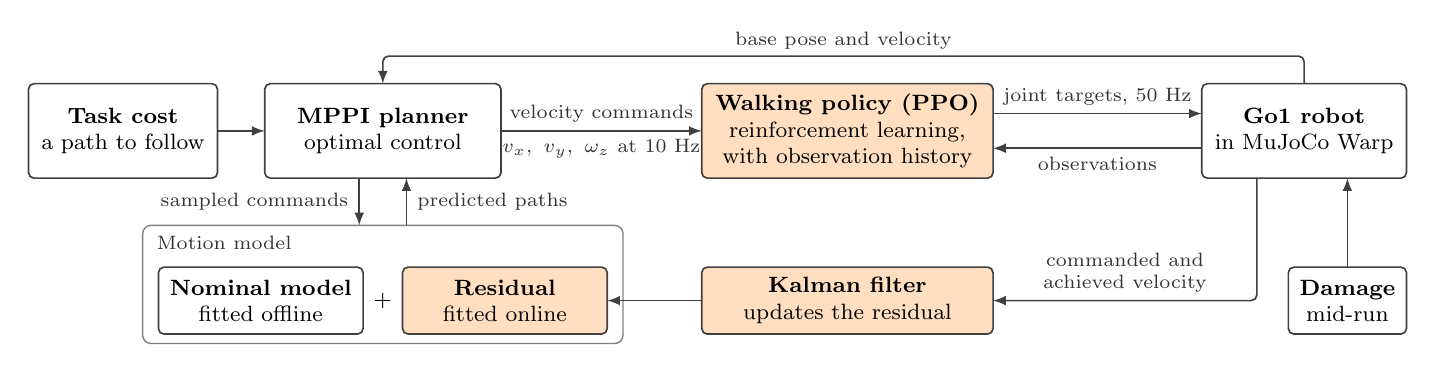
\begin{tikzpicture}[
    x=1cm, y=1cm,
    font=\footnotesize,
    box/.style={draw=black!75, line width=0.6pt, rounded corners=2pt,
      align=center, inner sep=2pt},
    adapts/.style={fill=orange!25},
    flow/.style={-latex, draw=black!75, line width=0.6pt, rounded corners=2pt},
    lab/.style={font=\scriptsize, text=black!80, align=center, inner sep=1.5pt},
  ]
  % The planner's motion model: a fixed part and a part fitted online.
  \draw[black!50, line width=0.5pt, rounded corners=3pt] (1.45, 0) rectangle (7.55, 1.5);
  \node[lab, anchor=north west] at (1.57, 1.42) {Motion model};
  \node at (4.5, 0.545) {$+$};

  % Boxes. The upper row is the control chain, left to right.
  \node[box, minimum width=2.4cm, minimum height=1.2cm] (task) at (1.2, 2.7) {\textbf{Task cost}\\a path to follow};
  \node[box, minimum width=3cm, minimum height=1.2cm] (mppi) at (4.5, 2.7) {\textbf{MPPI planner}\\optimal control};
  \node[box, adapts, minimum width=3.7cm, minimum height=1.2cm] (policy) at (10.4, 2.7) {\textbf{Walking policy (PPO)}\\reinforcement learning,\\with observation history};
  \node[box, minimum width=2.6cm, minimum height=1.2cm] (robot) at (16.2, 2.7) {\textbf{Go1 robot}\\in MuJoCo Warp};
  \node[box, minimum width=2.6cm, minimum height=0.85cm] (nominal) at (2.95, 0.545) {\textbf{Nominal model}\\fitted offline};
  \node[box, adapts, minimum width=2.6cm, minimum height=0.85cm] (residual) at (6.05, 0.545) {\textbf{Residual}\\fitted online};
  \node[box, adapts, minimum width=3.7cm, minimum height=0.85cm] (kalman) at (10.4, 0.545) {\textbf{Kalman filter}\\updates the residual};
  \node[box, minimum width=1.5cm, minimum height=0.85cm] (damage) at (16.75, 0.545) {\textbf{Damage}\\mid-run};

  % Arrows.
  \draw[flow] (2.4, 2.7) -- (3, 2.7);
  \draw[flow] (6, 2.7) -- (8.55, 2.7);
  \draw[flow] (12.25, 2.92) -- (14.9, 2.92);
  \draw[flow] (14.9, 2.48) -- (12.25, 2.48);
  \draw[flow] (4.2, 2.1) -- (4.2, 1.5);
  \draw[flow] (4.8, 1.5) -- (4.8, 2.1);
  \draw[flow] (16.2, 3.3) -- (16.2, 3.65) -- (4.5, 3.65) -- (4.5, 3.3);
  \draw[flow] (15.6, 2.1) -- (15.6, 0.545) -- (12.25, 0.545);
  \draw[flow] (8.55, 0.545) -- (7.35, 0.545);
  \draw[flow] (16.75, 0.97) -- (16.75, 2.1);

  % Arrow labels.
  \node[lab, anchor=south] at (7.275, 2.75) {velocity commands};
  \node[lab, anchor=north] at (7.275, 2.65) {$v_x,\ v_y,\ \omega_z$ at 10 Hz};
  \node[lab, anchor=south] at (13.575, 2.97) {joint targets, 50 Hz};
  \node[lab, anchor=north] at (13.575, 2.43) {observations};
  \node[lab, anchor=east] at (4.12, 1.8) {sampled commands};
  \node[lab, anchor=west] at (4.88, 1.8) {predicted paths};
  \node[lab, anchor=south] at (10.35, 3.68) {base pose and velocity};
  \node[lab, anchor=south] at (13.925, 0.595) {commanded and\\achieved velocity};
\end{tikzpicture}
}
%     \caption{The system. An MPPI planner sends velocity commands to a PPO
%       walking policy, which drives the simulated robot. The shaded parts adapt
%       online: the policy through its observation history, and the planner
%       through a residual on its motion model, updated by a Kalman filter.}
%   \end{figure}
%
% To get the figure as a PDF of its own, compile system_figure_standalone.tex.
% The picture is 17.5 cm wide and 4.0 cm high. All coordinates are in cm.
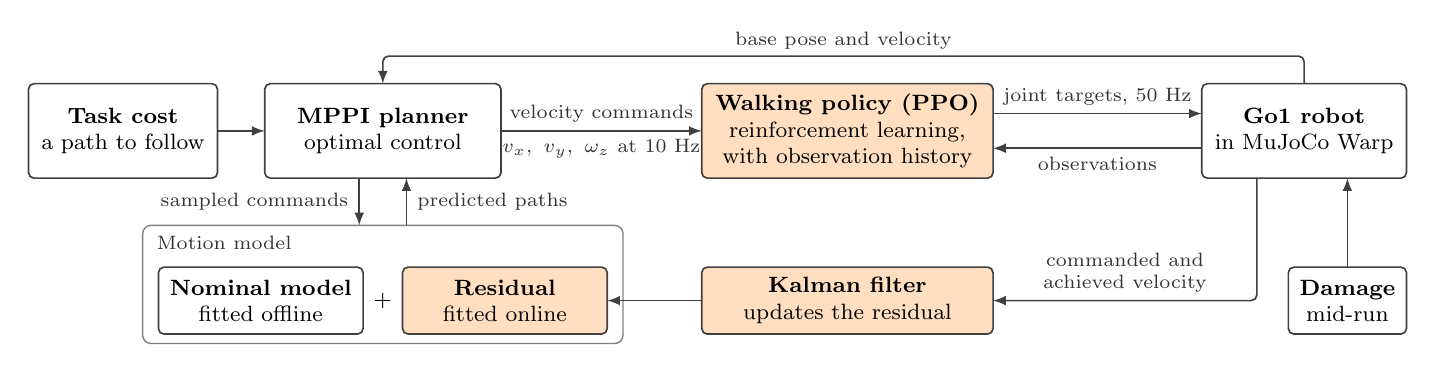
\begin{tikzpicture}[
    x=1cm, y=1cm,
    font=\footnotesize,
    box/.style={draw=black!75, line width=0.6pt, rounded corners=2pt,
      align=center, inner sep=2pt},
    adapts/.style={fill=orange!25},
    flow/.style={-latex, draw=black!75, line width=0.6pt, rounded corners=2pt},
    lab/.style={font=\scriptsize, text=black!80, align=center, inner sep=1.5pt},
  ]
  % The planner's motion model: a fixed part and a part fitted online.
  \draw[black!50, line width=0.5pt, rounded corners=3pt] (1.45, 0) rectangle (7.55, 1.5);
  \node[lab, anchor=north west] at (1.57, 1.42) {Motion model};
  \node at (4.5, 0.545) {$+$};

  % Boxes. The upper row is the control chain, left to right.
  \node[box, minimum width=2.4cm, minimum height=1.2cm] (task) at (1.2, 2.7) {\textbf{Task cost}\\a path to follow};
  \node[box, minimum width=3cm, minimum height=1.2cm] (mppi) at (4.5, 2.7) {\textbf{MPPI planner}\\optimal control};
  \node[box, adapts, minimum width=3.7cm, minimum height=1.2cm] (policy) at (10.4, 2.7) {\textbf{Walking policy (PPO)}\\reinforcement learning,\\with observation history};
  \node[box, minimum width=2.6cm, minimum height=1.2cm] (robot) at (16.2, 2.7) {\textbf{Go1 robot}\\in MuJoCo Warp};
  \node[box, minimum width=2.6cm, minimum height=0.85cm] (nominal) at (2.95, 0.545) {\textbf{Nominal model}\\fitted offline};
  \node[box, adapts, minimum width=2.6cm, minimum height=0.85cm] (residual) at (6.05, 0.545) {\textbf{Residual}\\fitted online};
  \node[box, adapts, minimum width=3.7cm, minimum height=0.85cm] (kalman) at (10.4, 0.545) {\textbf{Kalman filter}\\updates the residual};
  \node[box, minimum width=1.5cm, minimum height=0.85cm] (damage) at (16.75, 0.545) {\textbf{Damage}\\mid-run};

  % Arrows.
  \draw[flow] (2.4, 2.7) -- (3, 2.7);
  \draw[flow] (6, 2.7) -- (8.55, 2.7);
  \draw[flow] (12.25, 2.92) -- (14.9, 2.92);
  \draw[flow] (14.9, 2.48) -- (12.25, 2.48);
  \draw[flow] (4.2, 2.1) -- (4.2, 1.5);
  \draw[flow] (4.8, 1.5) -- (4.8, 2.1);
  \draw[flow] (16.2, 3.3) -- (16.2, 3.65) -- (4.5, 3.65) -- (4.5, 3.3);
  \draw[flow] (15.6, 2.1) -- (15.6, 0.545) -- (12.25, 0.545);
  \draw[flow] (8.55, 0.545) -- (7.35, 0.545);
  \draw[flow] (16.75, 0.97) -- (16.75, 2.1);

  % Arrow labels.
  \node[lab, anchor=south] at (7.275, 2.75) {velocity commands};
  \node[lab, anchor=north] at (7.275, 2.65) {$v_x,\ v_y,\ \omega_z$ at 10 Hz};
  \node[lab, anchor=south] at (13.575, 2.97) {joint targets, 50 Hz};
  \node[lab, anchor=north] at (13.575, 2.43) {observations};
  \node[lab, anchor=east] at (4.12, 1.8) {sampled commands};
  \node[lab, anchor=west] at (4.88, 1.8) {predicted paths};
  \node[lab, anchor=south] at (10.35, 3.68) {base pose and velocity};
  \node[lab, anchor=south] at (13.925, 0.595) {commanded and\\achieved velocity};
\end{tikzpicture}
}
%     \caption{The system. An MPPI planner sends velocity commands to a PPO
%       walking policy, which drives the simulated robot. The shaded parts adapt
%       online: the policy through its observation history, and the planner
%       through a residual on its motion model, updated by a Kalman filter.}
%   \end{figure}
%
% To get the figure as a PDF of its own, compile system_figure_standalone.tex.
% The picture is 17.5 cm wide and 4.0 cm high. All coordinates are in cm.
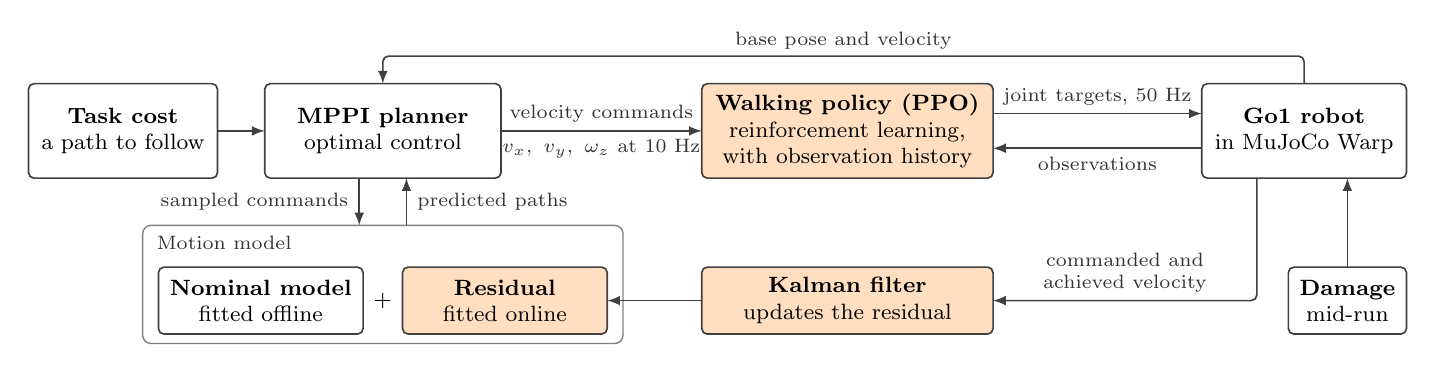
\begin{tikzpicture}[
    x=1cm, y=1cm,
    font=\footnotesize,
    box/.style={draw=black!75, line width=0.6pt, rounded corners=2pt,
      align=center, inner sep=2pt},
    adapts/.style={fill=orange!25},
    flow/.style={-latex, draw=black!75, line width=0.6pt, rounded corners=2pt},
    lab/.style={font=\scriptsize, text=black!80, align=center, inner sep=1.5pt},
  ]
  % The planner's motion model: a fixed part and a part fitted online.
  \draw[black!50, line width=0.5pt, rounded corners=3pt] (1.45, 0) rectangle (7.55, 1.5);
  \node[lab, anchor=north west] at (1.57, 1.42) {Motion model};
  \node at (4.5, 0.545) {$+$};

  % Boxes. The upper row is the control chain, left to right.
  \node[box, minimum width=2.4cm, minimum height=1.2cm] (task) at (1.2, 2.7) {\textbf{Task cost}\\a path to follow};
  \node[box, minimum width=3cm, minimum height=1.2cm] (mppi) at (4.5, 2.7) {\textbf{MPPI planner}\\optimal control};
  \node[box, adapts, minimum width=3.7cm, minimum height=1.2cm] (policy) at (10.4, 2.7) {\textbf{Walking policy (PPO)}\\reinforcement learning,\\with observation history};
  \node[box, minimum width=2.6cm, minimum height=1.2cm] (robot) at (16.2, 2.7) {\textbf{Go1 robot}\\in MuJoCo Warp};
  \node[box, minimum width=2.6cm, minimum height=0.85cm] (nominal) at (2.95, 0.545) {\textbf{Nominal model}\\fitted offline};
  \node[box, adapts, minimum width=2.6cm, minimum height=0.85cm] (residual) at (6.05, 0.545) {\textbf{Residual}\\fitted online};
  \node[box, adapts, minimum width=3.7cm, minimum height=0.85cm] (kalman) at (10.4, 0.545) {\textbf{Kalman filter}\\updates the residual};
  \node[box, minimum width=1.5cm, minimum height=0.85cm] (damage) at (16.75, 0.545) {\textbf{Damage}\\mid-run};

  % Arrows.
  \draw[flow] (2.4, 2.7) -- (3, 2.7);
  \draw[flow] (6, 2.7) -- (8.55, 2.7);
  \draw[flow] (12.25, 2.92) -- (14.9, 2.92);
  \draw[flow] (14.9, 2.48) -- (12.25, 2.48);
  \draw[flow] (4.2, 2.1) -- (4.2, 1.5);
  \draw[flow] (4.8, 1.5) -- (4.8, 2.1);
  \draw[flow] (16.2, 3.3) -- (16.2, 3.65) -- (4.5, 3.65) -- (4.5, 3.3);
  \draw[flow] (15.6, 2.1) -- (15.6, 0.545) -- (12.25, 0.545);
  \draw[flow] (8.55, 0.545) -- (7.35, 0.545);
  \draw[flow] (16.75, 0.97) -- (16.75, 2.1);

  % Arrow labels.
  \node[lab, anchor=south] at (7.275, 2.75) {velocity commands};
  \node[lab, anchor=north] at (7.275, 2.65) {$v_x,\ v_y,\ \omega_z$ at 10 Hz};
  \node[lab, anchor=south] at (13.575, 2.97) {joint targets, 50 Hz};
  \node[lab, anchor=north] at (13.575, 2.43) {observations};
  \node[lab, anchor=east] at (4.12, 1.8) {sampled commands};
  \node[lab, anchor=west] at (4.88, 1.8) {predicted paths};
  \node[lab, anchor=south] at (10.35, 3.68) {base pose and velocity};
  \node[lab, anchor=south] at (13.925, 0.595) {commanded and\\achieved velocity};
\end{tikzpicture}
}
%     \caption{The system. An MPPI planner sends velocity commands to a PPO
%       walking policy, which drives the simulated robot. The shaded parts adapt
%       online: the policy through its observation history, and the planner
%       through a residual on its motion model, updated by a Kalman filter.}
%   \end{figure}
%
% To get the figure as a PDF of its own, compile system_figure_standalone.tex.
% The picture is 17.5 cm wide and 4.0 cm high. All coordinates are in cm.
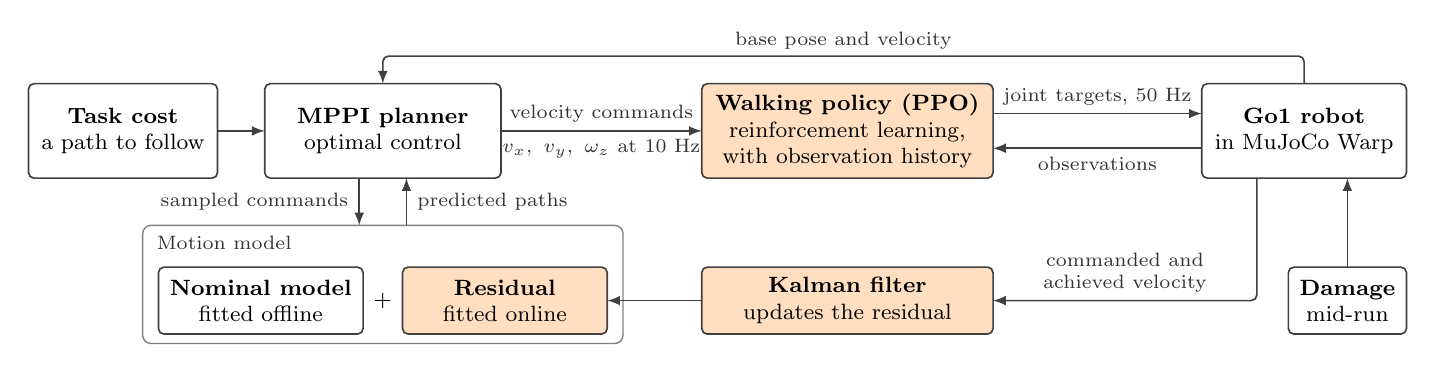
\begin{tikzpicture}[
    x=1cm, y=1cm,
    font=\footnotesize,
    box/.style={draw=black!75, line width=0.6pt, rounded corners=2pt,
      align=center, inner sep=2pt},
    adapts/.style={fill=orange!25},
    flow/.style={-latex, draw=black!75, line width=0.6pt, rounded corners=2pt},
    lab/.style={font=\scriptsize, text=black!80, align=center, inner sep=1.5pt},
  ]
  % The planner's motion model: a fixed part and a part fitted online.
  \draw[black!50, line width=0.5pt, rounded corners=3pt] (1.45, 0) rectangle (7.55, 1.5);
  \node[lab, anchor=north west] at (1.57, 1.42) {Motion model};
  \node at (4.5, 0.545) {$+$};

  % Boxes. The upper row is the control chain, left to right.
  \node[box, minimum width=2.4cm, minimum height=1.2cm] (task) at (1.2, 2.7) {\textbf{Task cost}\\a path to follow};
  \node[box, minimum width=3cm, minimum height=1.2cm] (mppi) at (4.5, 2.7) {\textbf{MPPI planner}\\optimal control};
  \node[box, adapts, minimum width=3.7cm, minimum height=1.2cm] (policy) at (10.4, 2.7) {\textbf{Walking policy (PPO)}\\reinforcement learning,\\with observation history};
  \node[box, minimum width=2.6cm, minimum height=1.2cm] (robot) at (16.2, 2.7) {\textbf{Go1 robot}\\in MuJoCo Warp};
  \node[box, minimum width=2.6cm, minimum height=0.85cm] (nominal) at (2.95, 0.545) {\textbf{Nominal model}\\fitted offline};
  \node[box, adapts, minimum width=2.6cm, minimum height=0.85cm] (residual) at (6.05, 0.545) {\textbf{Residual}\\fitted online};
  \node[box, adapts, minimum width=3.7cm, minimum height=0.85cm] (kalman) at (10.4, 0.545) {\textbf{Kalman filter}\\updates the residual};
  \node[box, minimum width=1.5cm, minimum height=0.85cm] (damage) at (16.75, 0.545) {\textbf{Damage}\\mid-run};

  % Arrows.
  \draw[flow] (2.4, 2.7) -- (3, 2.7);
  \draw[flow] (6, 2.7) -- (8.55, 2.7);
  \draw[flow] (12.25, 2.92) -- (14.9, 2.92);
  \draw[flow] (14.9, 2.48) -- (12.25, 2.48);
  \draw[flow] (4.2, 2.1) -- (4.2, 1.5);
  \draw[flow] (4.8, 1.5) -- (4.8, 2.1);
  \draw[flow] (16.2, 3.3) -- (16.2, 3.65) -- (4.5, 3.65) -- (4.5, 3.3);
  \draw[flow] (15.6, 2.1) -- (15.6, 0.545) -- (12.25, 0.545);
  \draw[flow] (8.55, 0.545) -- (7.35, 0.545);
  \draw[flow] (16.75, 0.97) -- (16.75, 2.1);

  % Arrow labels.
  \node[lab, anchor=south] at (7.275, 2.75) {velocity commands};
  \node[lab, anchor=north] at (7.275, 2.65) {$v_x,\ v_y,\ \omega_z$ at 10 Hz};
  \node[lab, anchor=south] at (13.575, 2.97) {joint targets, 50 Hz};
  \node[lab, anchor=north] at (13.575, 2.43) {observations};
  \node[lab, anchor=east] at (4.12, 1.8) {sampled commands};
  \node[lab, anchor=west] at (4.88, 1.8) {predicted paths};
  \node[lab, anchor=south] at (10.35, 3.68) {base pose and velocity};
  \node[lab, anchor=south] at (13.925, 0.595) {commanded and\\achieved velocity};
\end{tikzpicture}
